\documentclass[12pt,twoside,a4paper]{report}
\usepackage{etex}
% Select encoding of your inputs.
\usepackage[utf8]{inputenc}

% Make latex understand and use the typographic
% rules of the language used in the document.
\usepackage[english, danish]{babel}

% Use the vector font Latin Modern which is going
% to be the default font in latex in the future.
\usepackage{lmodern}

% Choose the font encoding
\usepackage[T1]{fontenc}

% Use colour in tables
\usepackage[table]{xcolor}
\usepackage{array}
\usepackage{multirow}

% load a colour package
\usepackage{xcolor}
\definecolor{aaublue}{RGB}{33,26,82}% dark blue

% The standard graphics inclusion package
\definecolor{white}{RGB}{255,255,255} % define color white
\usepackage{graphicx}
\usepackage{adjustbox}

% Set up how figure and table captions are displayed
\usepackage{caption}
\captionsetup{
  font=footnotesize,% set font size to footnotesize
  labelfont=bf % bold label (e.g., Figure 3.2) font
}

% Enable row combination in tables
\usepackage{multirow}

% Make space between table lines and text
\renewcommand{\arraystretch}{1.5}

% Make the standard latex tables look so much better
\usepackage{array,booktabs}

% Enable the use of frames around, e.g., theorems
% The framed package is used in the example environment
\usepackage{framed}
\usepackage{colortbl}
\usepackage{longtable}
\usepackage{xcolor}
\usepackage{textcomp}

%%%%%%%%%%%%%%%%%%%%%%%%%%%%%%%%%%%%%%%%%%%%%%%%
% Mathematics
%%%%%%%%%%%%%%%%%%%%%%%%%%%%%%%%%%%%%%%%%%%%%%%%
% Defines new environments such as equation,
% align and split 
\usepackage{amsmath}
\usepackage{relsize}
% Adds new math symbols
\usepackage{amssymb}
% Use theorems in your document
% The ntheorem package is also used for the example environment
% When using thmmarks, amsmath must be an option as well. Otherwise \eqref doesn't work anymore.
\usepackage[framed,amsmath,thmmarks]{ntheorem}
\usepackage{cancel}

%%%%%%%%%%%%%%%%%%%%%%%%%%%%%%%%%%%%%%%%%%%%%%%%
% Page Layout
%%%%%%%%%%%%%%%%%%%%%%%%%%%%%%%%%%%%%%%%%%%%%%%%
% Change margins, papersize, etc of the document
\usepackage[
  left=25mm,% left margin on an odd page %tidligere 25mm for baade right og left
  right=25mm,% right margin on an odd page
  top=35mm,
  ]{geometry}
  
% Modify how \chapter, \section, etc. look
% The titlesec package is very configureable
\usepackage{titlesec}
\makeatletter
\def\ttl@mkchap@i#1#2#3#4#5#6#7{%
    \ttl@assign\@tempskipa#3\relax\beforetitleunit
    \vspace{\@tempskipa}%<<<<<< REMOVE THE * AFTER \vspace
    \global\@afterindenttrue
    \ifcase#5 \global\@afterindentfalse\fi
    \ttl@assign\@tempskipb#4\relax\aftertitleunit
    \ttl@topmode{\@tempskipb}{%
        \ttl@select{#6}{#1}{#2}{#7}}%
    \ttl@finmarks  % Outside the box!
    \@ifundefined{ttlp@#6}{}{\ttlp@write{#6}}}
\makeatother

\titlespacing{\chapter}{0pt}{0pt}{10pt}
\titlespacing{\section}{0pt}{0pt}{-5pt}
\titlespacing{\subsection}{0pt}{8pt}{-5pt}
\titlespacing{\subsubsection}{0pt}{6pt}{-10pt}

\titleformat*{\section}{\normalfont\Large\bfseries\color{aaublue}}
\titleformat*{\subsection}{\normalfont\large\bfseries\color{aaublue}}
\titleformat*{\subsubsection}{\normalfont\normalsize\bfseries\color{aaublue}}

\usepackage{bookmark}
\usepackage{titlesec, blindtext, color}
%\color{gray75}{gray}{0.75}
\newcommand{\hsp}{\hspace{20pt}}
\titleformat{\chapter}[hang]{\Huge\bfseries}{\thechapter\hsp\textcolor{aaublue}{|}\hsp}{0pt}{\Huge\bfseries}

% Change the headers and footers
\usepackage{fancyhdr}
\setlength{\headheight}{15pt}
\pagestyle{fancy}
\fancyhf{} %delete everything
\renewcommand{\headrulewidth}{0pt} %remove the horizontal line in the header
\fancyhead[RO,LE]{\color{aaublue}\small\nouppercase\leftmark} %even page - chapter title
\fancyhead[LO]{}
\fancyhead[RE]{} 
\fancyhead[CE]{}
\fancyhead[CO]{}
\fancyfoot[RE,LO]{\thepage}
\fancyfoot[LE,RO]{B205} %page number on all pages
\fancyfoot[CE,CO]{}

% change first page of all chapters header and footer to fancy style
\makeatletter
\let\ps@plain\ps@fancy
\makeatother

% Do not stretch the content of a page. Instead,
% insert white space at the bottom of the page
\raggedbottom

% Enable arithmetics with length. Useful when typesetting the layout.
\usepackage{calc}

%%%%%%%%%%%%%%%%%%%%%%%%%%%%%%%%%%%%%%%%%%%%%%%%
% Bibliography
%%%%%%%%%%%%%%%%%%%%%%%%%%%%%%%%%%%%%%%%%%%%%%%%
%setting references (using numbers) and supporting i.a. Chicargo-style:
\usepackage{etex}
\usepackage{etoolbox}
\usepackage{keyval}
\usepackage{ifthen}
\usepackage{url}
\usepackage{csquotes}
\usepackage[backend=biber, url=true, doi=true, style=numeric, sorting=none]{biblatex}
\addbibresource{setup/bibliography.bib}

%%%%%%%%%%%%%%%%%%%%%%%%%%%%%%%%%%%%%%%%%%%%%%%%
% Misc
%%%%%%%%%%%%%%%%%%%%%%%%%%%%%%%%%%%%%%%%%%%%%%%%

%%% Enables the use FiXme refferences. Syntax: \fxnote{...} %%%
\usepackage[footnote, draft, english, silent, nomargin]{fixme}
%With "final" instead of "draft" an error will ocure for every FiXme under compilation.

%%% allows use of lorem ipsum (generate i.e. pagagraph 1 to 5 with \lipsum[1-5]) %%%
\usepackage{lipsum}

%%% Enables figures with text wrapped tightly around it %%%
\usepackage{wrapfig}

%%% Section debth included in table of contents (1 = down to sections) %%%
\setcounter{tocdepth}{1}

%%% Section debth for numbers (1 = down to sections) %%%
\setcounter{secnumdepth}{1}

\usepackage{tocloft}
\setlength{\cftbeforetoctitleskip}{0 cm}
\renewcommand{\cftpartpresnum}{Part~}
\let\cftoldpartfont\cftpartfont
\renewcommand{\cftpartfont}{\cftoldpartfont\cftpartpresnum}

%%%%%%%%%%%%%%%%%%%%%%%%%%%%%%%%%%%%%%%%%%%%%%%%
% Hyperlinks
%%%%%%%%%%%%%%%%%%%%%%%%%%%%%%%%%%%%%%%%%%%%%%%%

% Enable hyperlinks and insert info into the pdf
% file. Hypperref should be loaded as one of the 
% last packages
\usepackage{nameref}
\usepackage{hyperref}
\hypersetup{%
	%pdfpagelabels=true,%
	plainpages=false,%
	pdfauthor={Author(s)},%
	pdftitle={Title},%
	pdfsubject={Subject},%
	bookmarksnumbered=true,%
	colorlinks,%
	citecolor=aaublue,%
	filecolor=aaublue,%
	linkcolor=aaublue,% you should probably change this to black before printing
	urlcolor=aaublue,%
	pdfstartview=FitH%
}

% remove all indentations
\setlength\parindent{0pt}
\parskip 5mm
\usepackage{verbatim}

\definecolor{Gra}{RGB}{230,230,230}

%creates a nice-looking C#-text
\newcommand{\CC}{C\nolinebreak\hspace{-.05em}\raisebox{.3ex}{\scriptsize\text \#} }

%enables multi column lists
\usepackage{multicol}

%enables code-examples
\usepackage{listings}

\definecolor{coolblue}{RGB}{32,95,128}
\definecolor{mygreen}{rgb}{0,0.6,0}
\definecolor{mygray}{rgb}{0.5,0.5,0.5}
\definecolor{mymauve}{rgb}{0.58,0,0.82}
\usepackage{textcomp}
\definecolor{listinggray}{gray}{0.9}
\definecolor{lbcolor}{rgb}{0.9,0.9,0.9}

\lstset{
%  backgroundcolor=\color{white},   % choose the background color; you must add \usepackage{color} or \usepackage{xcolor}
%  basicstyle=\footnotesize,        % the size of the fonts that are used for the code
%  breakatwhitespace=false,         % sets if automatic breaks should only happen at whitespace
%  breaklines=true,                 % sets automatic line breaking
%  captionpos=t,                    % sets the caption-position to bottom
%  commentstyle=\color{mygreen},    % comment style
%  deletekeywords={...},            % if you want to delete keywords from the given language
%  escapeinside={\%*}{*)},          % if you want to add LaTeX within your code
%  extendedchars=true,              % lets you use non-ASCII characters; for 8-bits encodings only, does not work with UTF-8
%  frame=single,                    % adds a frame around the code
%  keepspaces=true,                 % keeps spaces in text, useful for keeping indentation of code (possibly needs columns=flexible)
%  keywordstyle=\color{blue},       % keyword style
%  language=C++,                 % the language of the code
%  morekeywords={*,...},            % if you want to add more keywords to the set
%  numbers=left,                    % where to put the line-numbers; possible values are (none, left, right)
%  numbersep=5pt,                   % how far the line-numbers are from the code
%  numberstyle=\tiny\color{mygray}, % the style that is used for the line-numbers
%  rulecolor=\color{black},         % if not set, the frame-color may be changed on line-breaks within not-black text (e.g. comments (green here))
%  showspaces=false,                % show spaces everywhere adding particular underscores; it overrides 'showstringspaces'
%  showstringspaces=false,          % underline spaces within strings only
%  showtabs=false,                  % show tabs within strings adding particular underscores
%  stepnumber=1,                    % the step between two line-numbers. If it's 1, each line will be numbered
%  stringstyle=\color{mymauve},     % string literal style
%  tabsize=2,                       % sets default tabsize to 2 spaces
%  title=\lstname                   % show the filename of files included with \lstinputlisting; also try caption instead of title
backgroundcolor=\color{lbcolor},
	tabsize=4,
	rulecolor=,
	language=C,
        basicstyle=\scriptsize,
        upquote=true,
        aboveskip={1.5\baselineskip},
        columns=fixed,
        showstringspaces=false,
        extendedchars=true,
        breaklines=true,
        prebreak = \raisebox{0ex}[0ex][0ex]{\ensuremath{\hookleftarrow}},
        frame=single,
        showtabs=false,
        numbers=left,
        captionpos=b,
        numbersep=5pt,
        numberstyle=\tiny\color{mygray},
        showspaces=false,
        showstringspaces=false,
        identifierstyle=\ttfamily,
        keywordstyle=\color[rgb]{0,0,1},
        commentstyle=\color[rgb]{0.133,0.545,0.133},
        stringstyle=\color[rgb]{0.627,0.126,0.941},
}

\usepackage{float}
\usepackage{caption}
\usepackage{subcaption}
\usepackage{siunitx}
\sisetup{decimalsymbol=comma}
\sisetup{detect-weight}

\usepackage{enumitem}
%\usepackage[citestyle=authoryear,natbib=true]{biblatex}

% Figures - TIKZ
\usepackage{tikz}
\usetikzlibrary{shapes,arrows}
\usepackage[americanresistors,americaninductors,americancurrents, americanvoltages]{circuitikz}

% Wall of text logo
\newcommand{\walloftextalert}[0]{\includegraphics[width=\textwidth]{walloftext.png}}

\usepackage{pdfpages}
\usepackage{lastpage}
\usepackage{epstopdf}

\setlength{\headheight}{21pt}

\hfuzz=\maxdimen
\tolerance = 10000
\hbadness  = 10000

\usepackage{siunitx}
\graphicspath{{./figures/}}% package inclusion and set up of the document

%%%%%%%%%%%%%%%%%%%%%%%%%%%%%%%%%%%%%%%%%%%%%%%%%%%%%
%             UNITS, EQUATIONS AND TEXT             %
%%%%%%%%%%%%%%%%%%%%%%%%%%%%%%%%%%%%%%%%%%%%%%%%%%%%%
%Units:
\newcommand{\unit}[1]{&& \left[\si{#1}\right]} %\newcommand{\unit}[1]{[\si{#1}]}             <<| Use these if you want equations to be
\newcommand{\unitWh}[1]{[\si{#1}]}             %\newcommand{\eq}[2]{&&\si{#1} &= \si{#2}&&}  <<| centered.. .. will appear scrambled
\newcommand{\numUnit}[1]{\ \si{#1}&}           %                                               | from one equation to the next though..
%Equation:                                     %                                               | and does not work with long equations.. :/
\newcommand{\eq}[2]{\si{#1} &= \si{#2}}
\newcommand{\arw}{&& &\Updownarrow&&}
%Text:
\newcommand{\tx}[1]{\text{#1}}
%Vectors
\renewcommand{\vec}[1]{\boldsymbol{\mathbf{#1}}}

%%%%%%%%%%%%%%%%%%%%%%%%%%%%%%%%%%%%%%%%%%%%%%%%%%%%%
%                  REFERENCES                       %
%%%%%%%%%%%%%%%%%%%%%%%%%%%%%%%%%%%%%%%%%%%%%%%%%%%%%

%Chapter
\newcommand{\Chapref}[1]{\emph{Chapter \ref{#1}}}
\newcommand{\chapref}[1]{\emph{chapter \ref{#1}}}
%Section
\newcommand{\Secref}[1]{\emph{Section \ref{#1}}}
\newcommand{\secref}[1]{\emph{section \ref{#1}}}
%subSection
\newcommand{\Subsecref}[1]{\emph{Subsection \ref{#1}}}
\newcommand{\subsecref}[1]{\emph{subsection \ref{#1}}}
%Appendix
\newcommand{\Appref}[1]{\emph{Appendix \ref{#1}}}
\newcommand{\appref}[1]{\emph{appendix \ref{#1}}}
%Listings
\newcommand{\Coderef}[1]{\emph{Listings: \ref{#1}}}
\newcommand{\coderef}[1]{\emph{listings: \ref{#1}}}
%Figure:
\newcommand{\Figref}[1]{\emph{Figure \ref{#1}}}
\newcommand{\figref}[1]{\emph{figure \ref{#1}}}
%Table:
\newcommand{\Tableref}[1]{\emph{Table \ref{#1}}}
\newcommand{\tableref}[1]{\emph{table \ref{#1}}}

%Expressions:
\newcommand{\Expr}[1]{\emph{Expression (\ref{#1})}}
\newcommand{\expr}[1]{\emph{expression (\ref{#1})}}

%Equations:
%1 equation:
\newcommand{\Eqref}[1]{\emph{Equation (\ref{#1})}}
\renewcommand{\eqref}[1]{\emph{equation (\ref{#1})}}
%2 equations:
\newcommand{\EqrefTwo}[2]{\emph{Equation (\ref{#1})} and \emph{(\ref{#2})}}
\newcommand{\eqrefTwo}[2]{\emph{equation (\ref{#1})} and \emph{(\ref{#2})}}
%3 equations:
\newcommand{\EqrefThree}[3]{\emph{Equation (\ref{#1})}, \emph{(\ref{#2})} and \emph{(\ref{#3})}}
\newcommand{\eqrefThree}[3]{\emph{equation (\ref{#1})}, \emph{(\ref{#2})} and \emph{(\ref{#3})}}
%4 equations:
\newcommand{\EqrefFour}[4]{\emph{Equation (\ref{#1})}, \emph{(\ref{#2})}, \emph{(\ref{#3})} and \emph{(\ref{#4})}}
\newcommand{\eqrefFour}[4]{\emph{equation (\ref{#1})}, \emph{(\ref{#2})}, \emph{(\ref{#3})} and \emph{(\ref{#4})}}
%5 equations:
\newcommand{\EqrefFive}[5]{\emph{Equation (\ref{#1})}, \emph{(\ref{#2})}, \emph{(\ref{#3})}, \emph{(\ref{#4})} and \emph{(\ref{#5})}}
\newcommand{\eqrefFive}[5]{\emph{equation (\ref{#1})}, \emph{(\ref{#2})}, \emph{(\ref{#3})}, \emph{(\ref{#4})} and \emph{(\ref{#5})}}
%6 equations:
\newcommand{\EqrefSix}[6]{\emph{Equation (\ref{#1})}, \emph{(\ref{#2})}, \emph{(\ref{#3})}, \emph{(\ref{#4})}, \emph{(\ref{#5})} and \emph{(\ref{#6})}}
\newcommand{\eqrefSix}[6]{\emph{equation (\ref{#1})}, \emph{(\ref{#2})}, \emph{(\ref{#3})}, \emph{(\ref{#4})}, \emph{(\ref{#5})} and \emph{(\ref{#6})}}
%7 equations:
\newcommand{\EqrefSeven}[7]{\emph{Equation (\ref{#1})}, \emph{(\ref{#2})}, \emph{(\ref{#3})}, \emph{(\ref{#4})}, \emph{(\ref{#5})}, \emph{(\ref{#6})} and \emph{(\ref{#7})}}
\newcommand{\eqrefSeven}[7]{\emph{equation (\ref{#1})}, \emph{(\ref{#2})}, \emph{(\ref{#3})}, \emph{(\ref{#4})}, \emph{(\ref{#5})}, \emph{(\ref{#6})} and \emph{(\ref{#7})}}% my new macros

\begin{document}
%%% Prereport %%%
\setlength\cftaftertoctitleskip{2pt}
\setlength\cftafterloftitleskip{6pt}
\setlength\cftafterlottitleskip{6pt}
\selectlanguage{english}
\title{Cubli}

%%% Frontmatter Settings %%%
\pagestyle{empty} %disable headers and footers
\pagenumbering{roman} %use roman page numbering in the frontmatter I II...
\fancyfoot[RE,LO]{15gr510} %page number on all pages
\fancyfoot[LE,RO]{\thepage}
\fancyhead[LE,LO,RE,RO]{}

%%% Introductory Formalities %%%
%\includepdf[pages={1}]{formalities/frontpage.pdf}
%\pdfbookmark[0]{Front Page}{label:forside}%
\begin{titlepage}
  \addtolength{\hoffset}{0.5\evensidemargin-0.5\oddsidemargin} %set equal margins on the frontpage - remove this line if you want default margins
  \noindent%
  \begin{tabular}{@{}p{\textwidth}@{}}
    \toprule[2pt]
    \midrule
    \vspace{0.2cm}
    \begin{center}
    \Huge{\textbf{
      Cubli % insert your title here
    }}
    \end{center}
    \begin{center}
      \Large{
      Dynamic Control of a Reaction Wheel Inverted Pendulum
      }
    \end{center}
    \vspace{0.2cm}\\
    \midrule
    \toprule[2pt]
  \end{tabular}
   \vspace{0.55 cm}
  \begin{figure}[!ht]
\centering
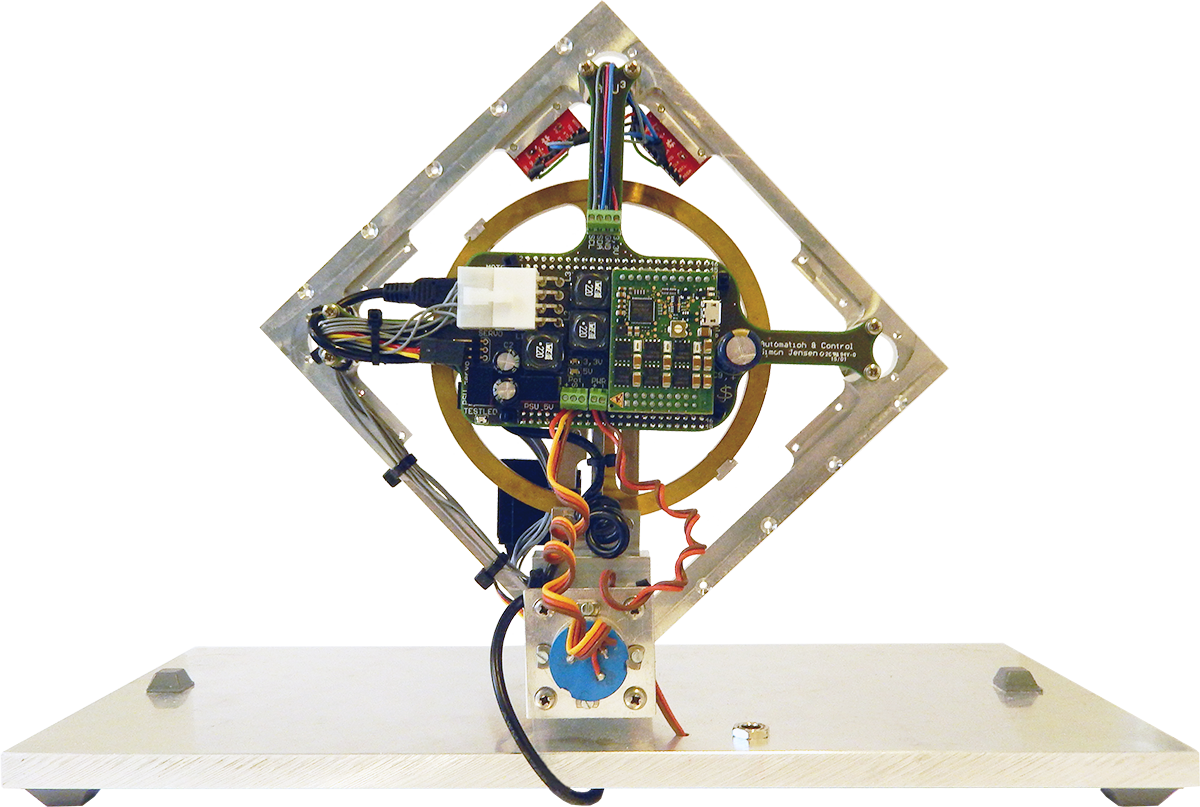
\includegraphics[width=0.95\textwidth]{figures/Cubli-1}
\label{fig:forside}
\end{figure}
  \vspace{0.6 cm}
  \begin{center}
    {\large
      6. Semester Project Report %Insert document type (e.g., Project Report)
    }\\
    \vspace{0.2cm}
    {\Large
      Group 16gr630%Insert your group name or real names here
    }
  \end{center}
  \begin{center}
  Aalborg University\\
  Electronic Engineering \& IT\\
  Fredrik Bajers Vej 7\\
  DK-9220 Aalborg
  \end{center}
\end{titlepage}

\clearpage
\pagestyle{fancy}
%\small
%\begin{figure}[H] 
%	\centering
%	\includegraphics[scale=0.38]{figures/Cubli-7}
%\end{figure}\vspace{-18pt}\begin{figure}[H] 
%	\centering
%	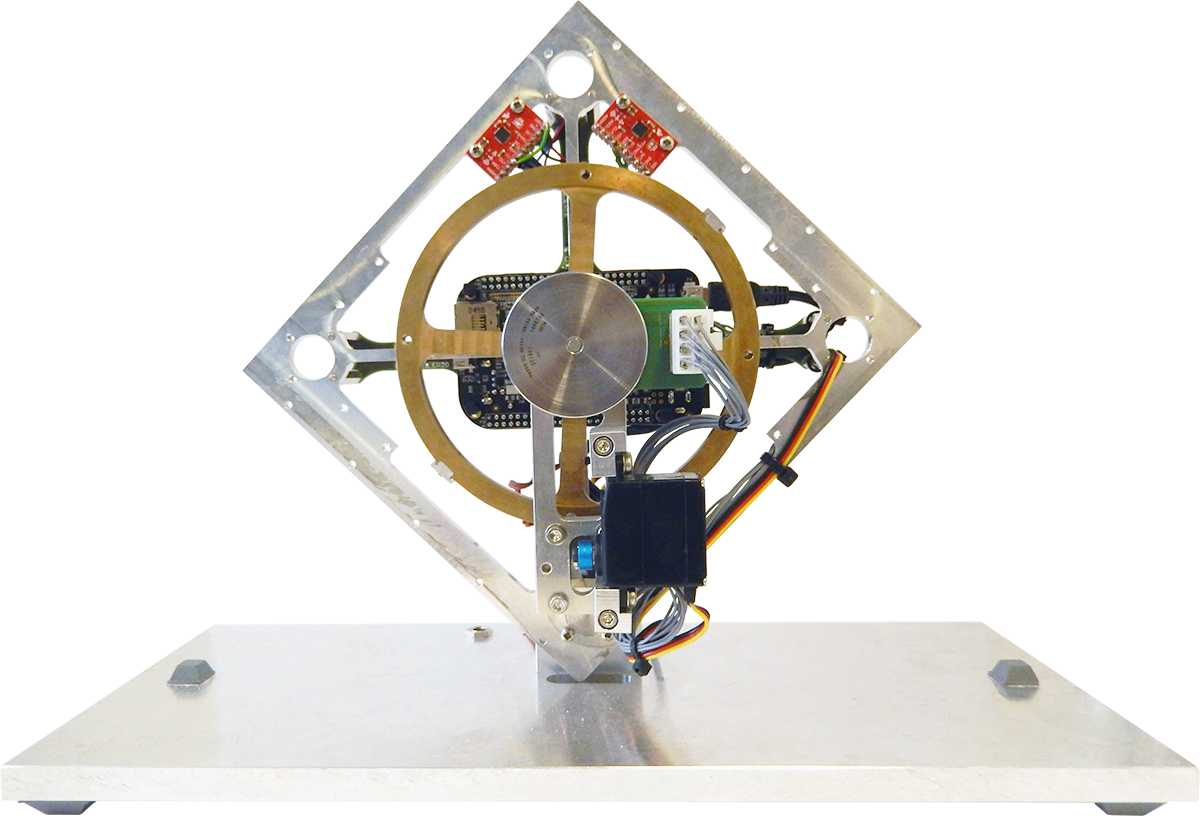
\includegraphics[scale=0.4]{figures/Cubli-2}
%\end{figure}\vspace{-18pt}\begin{figure}[H] 
%	\centering
%	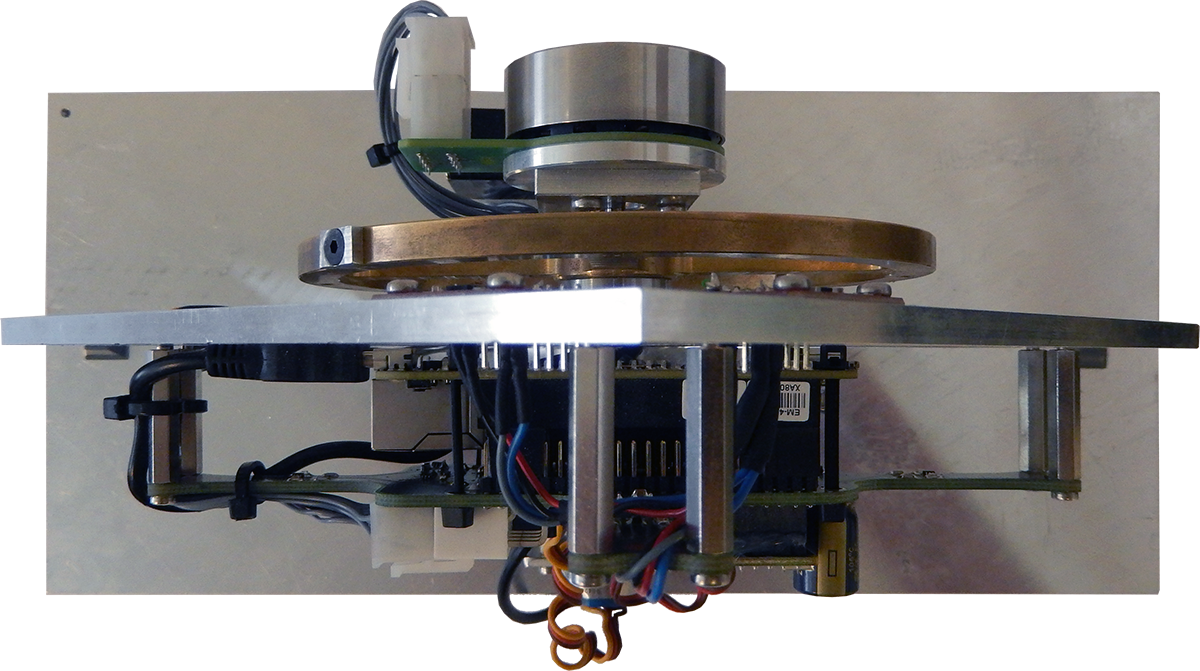
\includegraphics[scale=0.3, angle=180]{figures/Cubli-3}
%\end{figure}\vspace{-18pt}\begin{figure}[H] 
%	\centering
%	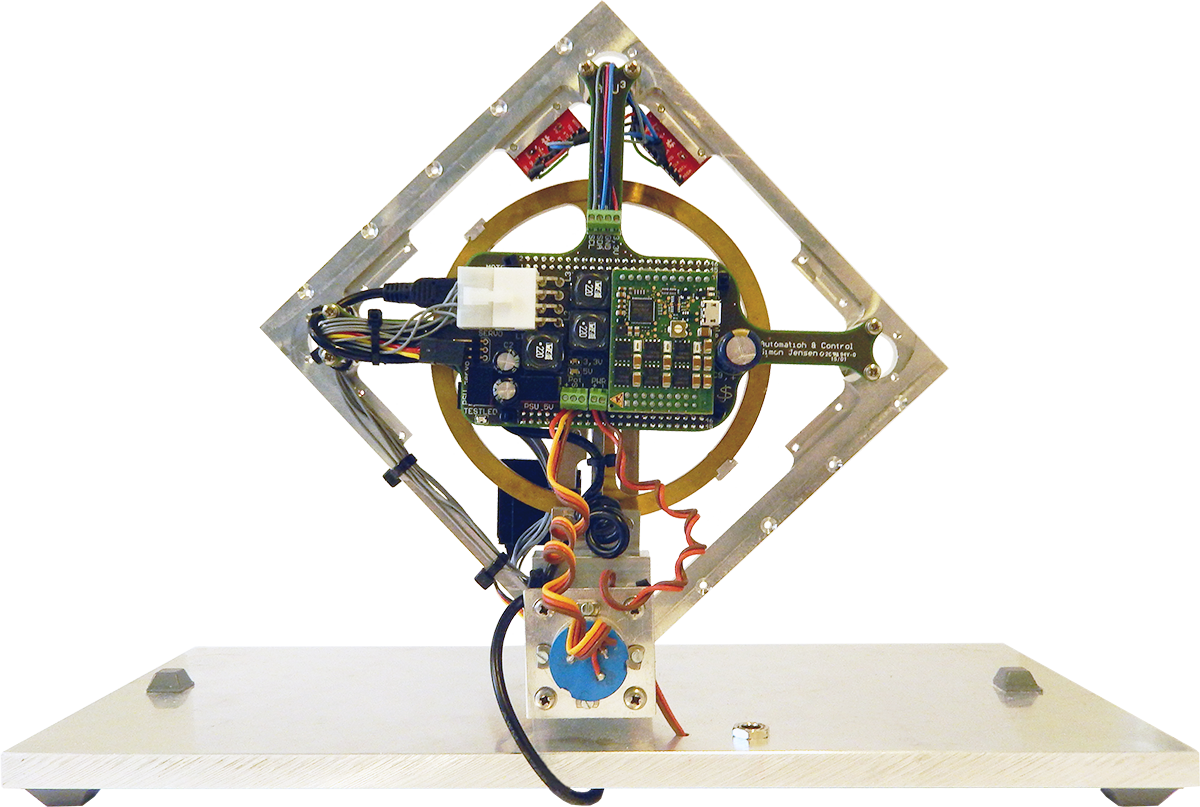
\includegraphics[scale=0.4, angle=180]{figures/Cubli-1}
%\end{figure}
\strut\vfill % push the content to the bottom of the page
\noindent Copyright \copyright{} Aalborg University 2016\par
\vspace{0.2cm}

\noindent This report is compiled in \LaTeX, originally developed by Leslie Lamport, based on Donald Knuth's \TeX. The main text is written in \emph{Latin Modern} pt 12, designed by Bogusław Jackowski and Janusz M. Nowacki. 
%The document is compiled via the website \url{www.overleaf.com}, an online collaborative based \LaTeX-editor with instant preview, which enables multiple persons to edit the document simultaneously.
Diagrams are made using Inkscape and Tikz.% Microsoft Visio. 
\clearpage
%\begin{document} 
\thispagestyle{empty}
\begin{titlepage}
\begin{nopagebreak}
{\samepage 

\begin{tabular}{r}
\parbox{\textwidth}{  \raisebox{-15mm}{
\includegraphics[height=3cm]{figures/aaulogo-en.png}}
\hfill \hspace{2cm} \parbox{8cm}{\begin{tabular}{l} %4.90
{\small \textbf{\textcolor{aaublue}{\colorbox{white}{6\textsuperscript{th} Semester, Bachelor Project}}}}\\
{\small \textbf{\textcolor{aaublue}{School of Information and}}}\\
{\small \textbf{\textcolor{aaublue}{Communication Technologies}}}\\ 
{\small \textbf{\textcolor{aaublue}{Electronics and IT}}}\\
{\small \textcolor{aaublue}{Fredrik Bajers Vej 7C}} \\
{\small \textcolor{aaublue}{9220 Aalborg}} \\
{\small \textcolor{aaublue}{\emph{http://www.sict.aau.dk/electronics-and-it}}}
\end{tabular}}}
\end{tabular}

\begin{tabular}{cc}
\parbox{7cm}{

\textbf{Title:}

Cubli:\\
Dynamic Control of a Reaction Wheel Inverted Pendulum\\ %\fxnote{Input project title}\\

\textbf{Theme:}

\small{
BSc Project (Control Engineering)\\
}


\parbox{8cm}{


\textbf{Project Period:}\\
P6, Spring 2016\\
01/02/2016 - 25/05/2016\\
   
\textbf{Project Group:}\\
630\\ %\fxnote{Input group number}
  
\textbf{Participants:}\\
Bjørn Kitz\\
Julien Br\'ehin\\
Mikael Sander\\
Niels Skov Vestergaard\\
Noelia Villarmarzo Arruñada\\

\textbf{Supervisor:}\\
John-Josef Leth\\ %\fxnote{Input supervisor}
Palle Andersen
}\\

\textbf{Prints:} 8\\
\textbf{Pages:}\\
\textbf{Appendices:}\\
\textbf{Attached:} 1 CD\\
\textbf{Concluded:} 25/05/2016\\

\vfill } &
\parbox{7cm}{
  \vspace{.15cm}
  \hfill
  \begin{tabular}{l}
  {\textbf{Synopsis}}\bigskip \\
  \fbox{
    \parbox{6.5cm}{\bigskip
     {\vfill{\small Nowadays, the inverted pendulum is used in many applications and it is a classic research area in control theory which is still active.

The aim of this project is to model and analyze the behavior of a reaction wheel inverted pendulum, in the form of a one-frame Cubli, and to design a controller capable of balance it in equilibrium position. 

Moreover, a solution for measuring its angular position using only internally mounted sensors is to be designed to be able to use it in a full Cubli. 

Finally, the performance of all the designs are tested in simulation and in the real prototype to ensure that they fulfill the needed requirements.
     \bigskip}}
     }}
   \end{tabular}}
\end{tabular}} %\vspace{1cm}

\textit{\phantom{A}Publication of this report's contents (including citation) without permission\\ \phantom{A}from the authors is prohibited}\\

\end{nopagebreak}
\end{titlepage}
%\end{document}
%%% Preface %%%
%\cleardoublepage
\textbf{\huge{Preface}}
\\
\\

\vspace{-12 pt}
\lipsum[3]\fxnote{Write prephase}

\textbf{Reading Instructions}
\vspace{-10 pt}
\begin{itemize}
\item[-] \lipsum[6]\fxnote{Write reading instructions}
\end{itemize}

%
\textbf{Text by:}\\
\vspace{-12 pt}
\begin{table}[H]
	\centering
		\begin{tabular}{c c c}
			\underline{\phantom{JAERJAERJAERJAERGO}} & \phantom{cookies} & \underline{\phantom{JAERJAERJAERJAERGO}} \\
			Bjørn Kitz			& \phantom{cookies} & Julien Br\'ehin		\\
			&&\\
			\underline{\phantom{JAERJAERJAERJAERGO}} & \phantom{cookies} & \underline{\phantom{JAERJAERJAERJAERGO}} \\
			Mikael Sander			& \phantom{cookies} & Niels Skov Vestergaard		\\
			&&\\
	    \multicolumn{3}{c}{\underline{\phantom{JAERJAERJAERJAERGO}}}\\
	    \multicolumn{3}{c}{Noelia Villarmarzo Arruñada}\\				
		\end{tabular}
\end{table}
\pagebreak

\pdfbookmark[0]{Table of Contents}{label: tableOfCentents}
\tableofcontents
\cleardoublepage


%%% Mainmatter Settings %%%
\pagenumbering{arabic} %use arabic page numbering in the mainmatter
\fancyfoot[RO,LE]{\thepage \text{ of} \pageref{LastPage}}
\fancyfoot[RE,LO]{15gr510}
\fancyhead[RE,LO]{}
\fancyhead[RE,LO]{\color{aaublue}\small\nouppercase\leftmark} %even page - chapter title
\pagestyle{fancy}

%%% Part 1 %%%
\part{Preanalysis}

%---------- Chapter 1 ---------------------------------------- Introduction
\chapter{Chapter 1}
We, as a group, wanted to work with an unlinear system for our bachelor project in control engineering. The choice fell on a form of inverted pendulum. It is a setup called Cubli.\fxnote{add picture of 3d cubli}
The Cubli is a cube that can jump up and balance on one of its sides or one of its corners.\cite{MGajamohan}
In this case the inverted pendulum setup is not controlled by a motor that moves the pendulum, but by a flywheel attached to the square frame. There is one for each of the three axis of motion. 
At AAU we have a one-dimensional setup, based on the Cubli idea. It consists of a metalframe with one flywheel. The idea is to balance the frame on one corner with the help of the flywheel by accelerating the wheel up and down.

\section{AAU Cubli}

\section{Section 2}
\subsection{Subsection 1.2.1}
\subsection{Subsection 1.2.2} %-------- For Overview, somtimes short headlines here works well

%---------- Chapter 2 ---------------------------------------- Design Considerations
\chapter{Design Considerations}\label{chap:designConsiderations}
% - Mechanical description of 3 dimensional cubli (focus: control)
%     - jump up on side
%     - jump up on corner 
%     - balancing on side
%     - balancing on corner
% - What have other cubli-makers achieved
%     - balance deviation (if moved x degrees away from equilibrium
%                          point - for how big x can it still find
%                          its equilibrium again)
%     - corner balance (duration?)
%     - general on stability
%         - Different slopes
%     - moving (rolling)
%     - spin

From the introduced applications both in modular robot design as well as planetary or asteroid exploration, a high controllability Cubli design is desired.
In a realization of a full functioning Cubli, different considerations regarding design and overall functionalities must be taken into account. Later in this chapter restrictions are considered regarding the features to implement in this project.

% The setup for this project is given by the university, which means that some considerations must be taken into account when modelling the system and designing a controller to balance it.

% The full Cubli setup is a 3 dimensional cube, whose structure is a metallic frame. Inside the frame, three reaction wheels are mounted and driven by DC motors and a brake system and additionally there are different kind of sensors inside the frame, that are used to determine the position of the Cubli.
% %\fxnote{Look in source material what kind of sensors the cubli is using}

% The system is controlled by the use of reaction wheels, which make it able to balance on a side or a corner and to jump up from rest position when braking the wheels. It is also possible to make it move in one direction, if the control of the wheels is combined.% At this point, the Cubli can be considered a cube robot.\\

% On the other hand, the working setup that exists at Aalborg University (AAU) is composed by one of the sides of the 3D cube. One of the most important characteristics is that one of its corners is attached to a base plate. This feature limits the number of movements the Cubli can do, as it can only be balanced in one direction along a vertical plane.

% Since all the hardware is already built, the goal of the project is focused on deriving the model of the system, simulating it to compare it with the real Cubli and, moreover, on designing a controller which is able to balance it in the equilibrium position.

%At Aalborg University (AAU), there exists a working setup of a one-dimensional Cubli. The overall goals of this semester are to make a model of a system, to simulate this model and then to design and implement a controller for that system. Students on this semester are encouraged to work with pre-made setups, since the focus is rather on the control engineering than the hardware solution.\fxnote{moved the section directly from introduction. Will need a top to catch the previous chapter}


%---------- Chapter 3 ---------------------------------------- Requirements
%\section{Design Limitations}
The working setup that exists at Aalborg University (AAU) is composed by one of the sides of the 3D cube.

Since all the hardware is already build, the goal of the project is focus on deriving the model of the system, simulate it to compare it with the real Cubli and design a controller capable of balance it in the equilibrium position.

One important characteristic is that one of its corners is attached to a base plate. This feature limits the number of movements the Cubli can do, as it can only be balance in one direction.

Another important limitation is given by the maximum current that the motor can provide which conditions the maximum starting angle that it can have with respect to equilibrium position. As can be seen in \figref{limitationTorque}, if the initial angle is different from 0 rad both the mass of the frame ans the mass of the wheel exert an initial torque to the system. This must be overcame by the motor in order to the Cubli not to fall.
%
\begin{figure}[H] 
	\centering
	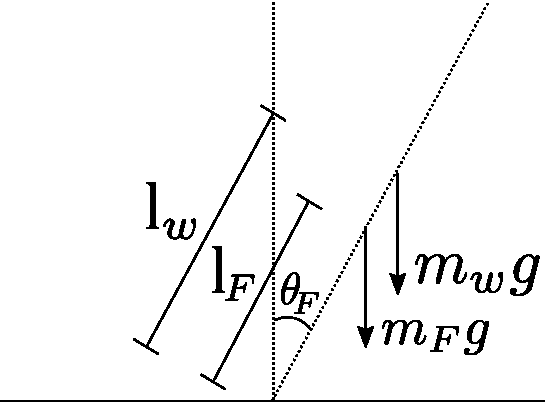
\includegraphics[scale=0.65]{figures/limitationTorque}
	\caption{Force acting on the system that create an initial torque}
	\label{limitationTorque}
\end{figure}

The minimum torque that the motor must apply is give by \eqref{minTorque}.
%
\begin{flalign}
	\eq{T} { (m_F \cdot l_F + m_w \cdot l_w) \cdot g \cdot sin(\theta_F)} \unit{N\cdot m}
	\label{minTorque}
\end{flalign}

Since the torque is restricted by the characteristics of the motor and the control board, the maximum initial angle is derived in \eqref{maxAngle}.
%
\begin{flalign}
	\eq{\theta_F} { asin\left(\frac{T}{(m_F \cdot l_F + m_w \cdot l_w) \cdot g}\right)} \unit{N\cdot m}
	\label{maxAngle}
\end{flalign}
%
Substituding the values of the maximum torque (see section \ref{sec:Motor}) and the parameters of the Cubli (see section \ref{sec:Param}) the maximum starting angle is \si{0,2024\ rad}.

\fxnote{The maximum angle may should be explained after the modeling and the estimation of parameters}
%At Aalborg University (AAU), there exists a working setup of a one-dimensional Cubli. The overall goals of this semester are to make a model of a system, to simulate this model and then to design and implement a controller for that system. Students on this semester are encouraged to work with pre-made setups, since the focus is rather on the control engineering than the hardware solution.\fxnote{moved the section directly from introduction. Will need a top to catch the previous chapter}



%%% Part 2 %%%
\part{Design \& Implementation}
%---------- Chapter 4 ---------------------------------------- Modelling
\chapter{System Description}
One-frame Cubli is a non-linear unstable system which is capable of laying on one of its corners as long as it is properly controlled, using the inertia created in the reaction wheel present in the setup.

This system is composed by several hardware parts, listed in the following table. \fxnote{insert correct part names} \fxnote{Include picture of the real model, mark all the parts in the picture}

\begin{table}[H]
	\begin{tabular}{|l|p{4.5cm}|}
		\hline %-----------------------------------------------------------------------------------
		\textbf{No.} &\textbf{Part} 			\\
		\hline %-----------------------------------------------------------------------------------
		1            & Frame           			\\
		\hline %-----------------------------------------------------------------------------------
		2            & Reaction wheel      		\\
		\hline %-----------------------------------------------------------------------------------
		3            & Controller (BeagleBone)  \\
		\hline %-----------------------------------------------------------------------------------
		4            & Potentiometer			\\
		\hline %-----------------------------------------------------------------------------------
		5            & IMU          			\\
		\hline %-----------------------------------------------------------------------------------
		6            & Brushless DC-motor   	\\
		\hline %-----------------------------------------------------------------------------------
		7            & Motor control board     	\\
		\hline %-----------------------------------------------------------------------------------
		8            & Jump brake		    	\\
		\hline %-----------------------------------------------------------------------------------
	\end{tabular}
	\caption{Main parts of the Cubli setup}
\label{TableAAUCubliComponent}
\end{table}

%A mechanical drawing of the Cubli showing angles and coordinate system conventions is seen in \figref{cubliMechanical}.

%\begin{figure}[H]
%  \centering
%  \includegraphics[scale=.5]{figures/cubliMechanical}
%  \caption{Mechanical drawing of the Cubli, including angle ang coordinate system conventions}
%  \label{cubliMechanical}
%\end{figure} 

The Cubli is split up into its two moving parts as seen in \figref{freeBodyFrame} and \figref{freeBodyWheel}.

  \begin{minipage}{\linewidth}
  	\begin{minipage}{0.45\linewidth}
  		\begin{figure}[H]
  			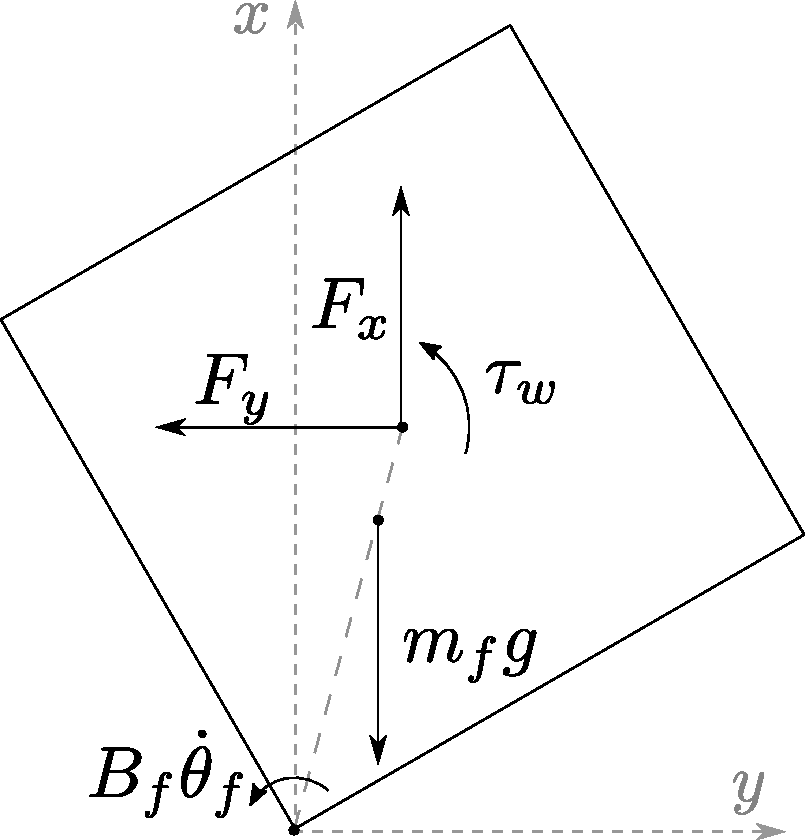
\includegraphics[scale=.5]{figures/freeBodyFrame}
  			\centering
  			\captionsetup{justification=centering}
  			\captionof{figure}{\\Free body diagram of the frame of the cubli}
  			\label{freeBodyFrame}
  		\end{figure}\vspace{-5mm}
  	\end{minipage}
  	\hspace{0.03\linewidth}
  	\begin{minipage}{0.45\linewidth}
  		\begin{figure}[H]
  			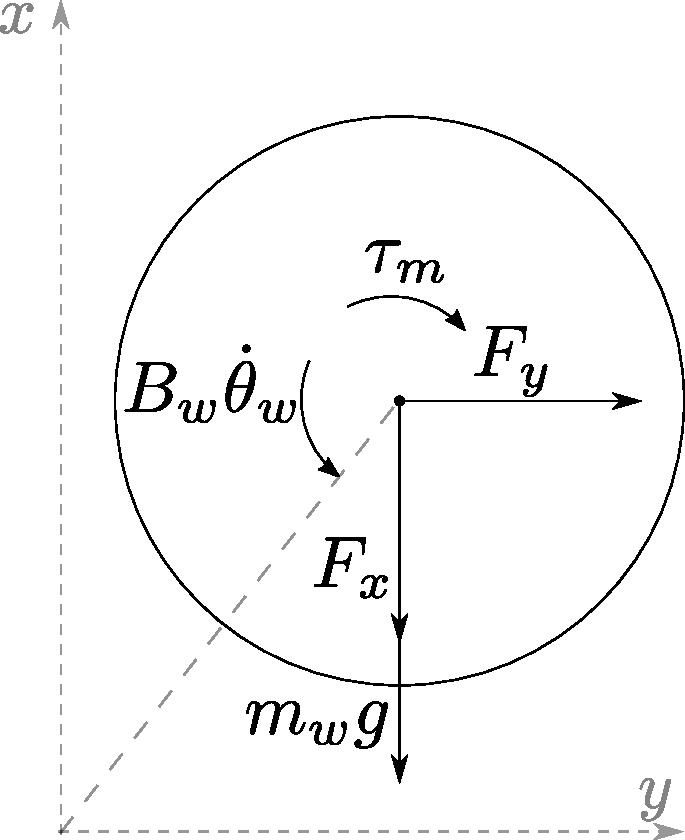
\includegraphics[scale=.53]{figures/freeBodyWheel}
  			\centering
  			\captionsetup{justification=centering}
  			\captionof{figure}{\\Free body diagram of the reaction wheel of the cubli}
  			\label{freeBodyWheel}
  		\end{figure}\vspace{-5mm}
  	\end{minipage}
  \end{minipage}

The equation for the frame is deduced from the \figref{freeBodyFrame}.
\begin{flalign}
  \eq{J_F \vec{\ddot{\theta}_F}} { -B_F \vec{\dot{\theta}_F} + \vec{l_F} \times (m_F\cdot \vec{g}) + \vec{l_w} \times \vec{F} - \vec{\tau_m} + B_w \vec{\dot{\theta}_w}} \unit{N\cdot m}
  \label{frameModelEq}
\end{flalign}
%
\hspace{6mm} Where:\\
\begin{tabular}{ p{1cm} l l l}
& \si{J_F} 					    	   & is the inertia of the frame                          &\unitWh{kg \cdot m^2} \\
& \si{\vec{\ddot{\theta}_F}} & is the angular acceleration of the frame             &\unitWh{rad \cdot s^{-2}} \\
& \si{B_F} 	                 & is the friction coefficient of the frame             &\unitWh{N \cdot m \cdot s \cdot rad^{-1}} \\
& \si{\vec{\dot{\theta}_F}}  & is the angular velocity of the frame                 &\unitWh{rad \cdot s^{-1}} \\
& \si{\vec{l_F}}             & is the length to center of mass of the frame         &\unitWh{m} \\
& \si{m_F}                   & is the mass of the frame                             &\unitWh{kg} \\
& \si{\vec{g}}							 & is the gravitational acceleration                    &\unitWh{m\cdot s^{-2}} \\
& \si{\vec{l_w}}             & is the length to center off mass of the wheel        &\unitWh{m} \\
& \si{\vec{F}}				  	   & is the force delivered to the frame from the wheel   &\unitWh{N} \\
& \si{\vec{\tau_m}} 	       & is the torque delivered by the motor        &\unitWh{N \cdot m} \\
& \si{B_w} 	                 & is the friction coefficient of the wheel             &\unitWh{N \cdot m \cdot s \cdot rad^{-1}} \\
& \si{\vec{\dot{\theta}_w}}  & is the angular velocity of the wheel with respect to the frame                 &\unitWh{rad \cdot s^{-1}} \\
\end{tabular}

The following equation is then derived from \figref{freeBodyWheel}:
\begin{flalign}
  \eq{ J_w (\ \vec{\ddot{\theta}_F} + \vec{\ddot{\theta}_w}\ ) } { \vec{\tau_m} - B_w \vec{\dot{\theta}_w }} \unit{N\cdot m }
  \label{tauW}
\end{flalign}
\hspace{6mm} Where:\\
\begin{tabular}{ p{1cm} l l l}
& \si{J_w} 					    	   & is the inertia of the wheel                          &\unitWh{kg \cdot m^2} \\
& \si{\vec{\ddot{\theta}_w}} & is the angular acceleration of the wheel with respect to the frame             &\unitWh{rad \cdot s^{-2}} \\
\end{tabular}

In \eqref{frameModelEq} the term \si{\vec{l_w} \times \vec{F}} describes the torque delivered from the wheel to the frame, as it acts around the pivot corner of the frame. The vector \si{\vec{F}} is decomposed into to forces paralell to the axes, \si{F_x} and \si{F_y}, as seen on \figref{freeBodyFrame} and \figref{freeBodyWheel}. To be able to apply Newton's Second Law, expressions for both the x- and y-coordinate describing the position of the center of mass of the wheel are found.
%
\begin{flalign}
  \eq{x} { l_w \cdot cos( \theta_F ) } \unit{ m }\\
  \eq{y} { l_w \cdot sin( \theta_F ) } \unit{ m }
  \label{xyCoordinate}
\end{flalign}
%
According to Newton's 2nd law of motion, \si{\sum F = m \cdot a}. Then to find \si{F_x} and \si{F_y}, the acceleration of the point at center of mass of the wheel must be known for both the x- and the y-direction. To achieve this the derivatives of the expressions for x and y in \eqref{xyCoordinate} are derived.
%
\begin{flalign}
  \eq{\dot{x}} { -l_w \cdot sin( \theta_F )\ \dot{\theta}_F } \unit{ m\cdot s^{-1} }\\
  \eq{\ddot{x}} { -l_w \cdot cos( \theta_F )\ {\dot{\theta}_F}^{\ \ 2} - l_w \cdot sin( \theta_F ) \ddot{\theta}_F } \unit{ m\cdot s^{-2} }
  \label{xCoordinateDerivatives}
\end{flalign}
%
\begin{flalign}
  \eq{\dot{y}} { l_w \cdot cos( \theta_F )\ \dot{\theta}_F } \unit{ m\cdot s^{-1} }\\
  \eq{\ddot{y}} { -l_w \cdot sin( \theta_F )\ {\dot{\theta}_F}^{\ \ 2} + l_w \cdot cos( \theta_F )\ \ddot{\theta}_F } \unit{ m\cdot s^{-2} }
  \label{yCoordinateDerivatives}
\end{flalign}
%
\Eqref{xCoordinateDerivatives} and \eqref{yCoordinateDerivatives} can now be used with Newton's 2nd law of motion, while also taking gravity into account in sum of forces, to derive \si{F_x} and \si{F_y}.
%
\begin{flalign}
  \eq{ -F_x -m_w \cdot g }{ m_w \cdot \ddot{x} } &\nonumber\\
  \eq{ F_x }{ - m_w \cdot \ddot{x} - m_w \cdot g} &\nonumber\\
  \eq{ F_x }{ m_w \cdot (\  l_w \cdot cos( \theta_F )\ {\dot{\theta}_F}^{\ \ 2} + l_w \cdot sin( \theta_F )\ \ddot{\theta}_F \ ) - m_w \cdot g} \unit{N}
  \label{Fx}
\end{flalign}
%
\begin{flalign}
  \eq{ -F_y }{ m_w \cdot \ddot{y} } & \nonumber\\
  \eq{ F_y }{ -m_w \cdot (\ -l_w \cdot sin( \theta_F )\ {\dot{\theta}_F}^{\ \ 2} + l_w \cdot cos( \theta_F )\ \ddot{\theta}_F\ ) } & \nonumber\\
  \eq{ F_y }{ m_w \cdot (\ l_w \cdot sin( \theta_F )\ {\dot{\theta}_F}^{\ \ 2} - l_w \cdot cos( \theta_F )\ \ddot{\theta}_F\ ) } \unit{N}
  \label{Fy}
\end{flalign}

The original objective was to evaluate the term \si{\vec{l_w} \times \vec{F}} in \eqref{frameModelEq}. Since the expressions for the two forces, \si{F_x} and \si{F_y}, that compose the vector \si{\vec{F}}, are found in \eqrefTwo{Fx}{Fy}, the vector product from \eqref{frameModelEq} is evaluated.

\begin{flalign}
  \si{\vec{l_w} \times \vec{F}} &=
    \begin{vmatrix}
      \ \si{\vec{\hat{i}}}                & \si{\vec{\hat{j}}}               & \si{\vec{\hat{k}}} \ \ \ \\ 
      \ \si{ l_w \cdot cos( \theta_F ) }  & \si{ l_w \cdot sin( \theta_F ) } & 0                  \ \ \ \\ 
      \ \si{ F_x }                        & \si{ F_y }                      & 0                  \ \ \  
    \end{vmatrix} \unit{N\cdot m}\\ \nonumber \\
  \si{ \vec{l_w} \times \vec{F} } &= 
    \begin{bmatrix}
      \ \si{ ( l_w \cdot sin( \theta_F) \cdot 0 - 0 \cdot F_y ) } \ \ \ \\
      \ \si{ ( l_w \cdot cos( \theta_F )\cdot 0 + 0 \cdot F_x  ) } \ \ \ \\
      \ \si{ ( l_w \cdot cos( \theta_F )\cdot F_y - l_w \cdot sin( \theta_F )\cdot F_x ) }
    \end{bmatrix} \unit{N\cdot m} \\ \nonumber\\
  \si{ \vec{l_w} \times \vec{F} } &= \si{ 0 \cdot \hat{i} + 0 \cdot \hat{j} + ( l_w \cdot cos( \theta_F )\cdot (m_w \cdot (\ l_w \cdot sin( \theta_F )\ {\dot{\theta}_F}^{\ \ 2} - l_w \cdot cos( \theta_F )\ \ddot{\theta}_F\ ))} \nonumber \\
  &\ \ \ \ \si{- l_w \cdot sin( \theta_F )\cdot (m_w \cdot (\  l_w \ cos( \theta_F )\ {\dot{\theta}_F}^{\ \ 2} + l_w \cdot sin( \theta_F )\ \ddot{\theta}_F \ )} \nonumber \\
  &\ \ \ \ \si{- m_w \cdot g) ) \cdot \hat{k}} \unit{N \cdot m}\\ \nonumber\\
  \eq{ \vec{l_w} \times \vec{F} }{ ({-l_w}^2 \cdot m_w \ddot{\theta}_F \ (cos^2(\theta_F) + sin^2(\theta_F)) + l_w\cdot sin(\theta_F)\ m_w \cdot g ) \cdot \hat{k}} \unit{N \cdot m}\\ \nonumber\\
  \eq{ \vec{l_w} \times \vec{F} }{ (-{l_w}^2 \cdot m_w \ddot{\theta}_F + l_w\ sin(\theta_F)\ m_w \cdot g ) \cdot \hat{k}} \unit{N \cdot m}
  \label{vectorDecomposition3}
\end{flalign}

Since all torques only have a z-coordinate, \eqref{vectorDecomposition3} is inserted in \eqref{frameModelEq}, without vector-notation. Note that \si{\vec{l_F} \times (m_F\cdot \vec{g}) = (m_F \cdot l_F \cdot g \cdot sin(\theta_F)) \cdot \hat{k} }.
%
\begin{flalign}
	\si{J_F \cdot \ddot{\theta}_F} &= \si{- B_F \cdot \dot{\theta}_F + m_F \cdot l_F \cdot g \cdot sin(\theta_F)} \nonumber\\ 
	&\ \ \ \ \si{- m_w \cdot {l_w}^{2} \cdot \ddot{\theta}_F + m_w \cdot l_w  \cdot g \cdot sin(\theta_F) - \tau_m + B_w \cdot \dot{\theta}_w} \unit{N\cdot m}
\label{FrameEq2}
\end{flalign}
%
\begin{flalign}
	\eq{(J_F+m_w \cdot {l_w}^{2}) \cdot \ddot{\theta}_F} {- B_F \cdot \dot{\theta}_F + (m_F \cdot l_F + m_w \cdot l_w) \cdot g \cdot sin(\theta_F) - \tau_m + B_w \cdot \dot{\theta}_w} \unit{N\cdot m}
\label{FrameEq3}
\end{flalign}

Isolating \si{\ddot{\theta}_F} from \eqref{FrameEq3} gives the final expression for the rotational acceleration of the frame.
\begin{flalign}
	\eq{\ddot{\theta}_F} {\frac{- B_F \cdot \dot{\theta}_F + (m_F \cdot l_F + m_w \cdot l_w) \cdot g \cdot sin(\theta_F) - \tau_m + B_w \cdot \dot{\theta}_w}{J_F + m_w \cdot {l_w}^{2}}}  \unit{rad \cdot s^{-1}} 
\label{FrameEqFinal}
\end{flalign}

Once the acceleration of the frame is described by \eqref{FrameEqFinal} it is possible to derive an expression for the angular acceleration of the wheel with respect to its axis from \eqref{tauW}.
\begin{flalign}
	\eq{\ddot{\theta}_w} {\frac{\tau_m - B_w \cdot \dot{\theta}_w}{J_w} - \ddot{\theta}_F} \unit{rad \cdot s^{-1}} 
\label{WheelRotEq2}
\end{flalign}

Substituting \si{\ddot{\theta}_F} by the expression for the angular acceleration of the frame (\eqref{FrameEqFinal}) into \eqref{WheelRotEq2} gives the final description for \si{\ddot{\theta}_w}, as shown in \eqref{WheelRotEqFinal}.
\begin{flalign}
	\si{\ddot{\theta}_w} &= \si{\frac{\tau_m - B_w \cdot \dot{\theta}_w}{J_w}}\nonumber\\ 
	&\ \ \ \ \si{- \frac{(m_F \cdot l_F + m_w \cdot l_w) \cdot g \cdot sin(\theta_F) - \tau_m + B_w \cdot \dot{\theta}_w - B_F \cdot \dot{\theta}_F}{J_F+m_w \cdot {l_w}^{2}}} \unit{rad \cdot s^{-1}}
\label{WheelRotEq3}
\end{flalign}
%
\begin{flalign}
	\si{\ddot{\theta}_w} &= \si{\frac{(J_w+J_F+{l_w}^{2} \cdot m_w) \cdot (\tau_m - B_w \cdot \dot{\theta}_w)}{J_w \cdot (J_F+m_w \cdot {l_w}^{2})}}\nonumber\\ 
	&\ \ \ \ \si{- \frac{(m_F \cdot l_F + m_w \cdot l_w) \cdot g \cdot sin(\theta_F) - B_F \cdot \dot{\theta}_F}{J_F+m_w \cdot {l_w}^{2}}} \unit{rad \cdot s^{-1}} 
\label{WheelRotEqFinal}
\end{flalign}             %-------- Model
\section{Linearization of the Model}
Now that a model of the Cubli frame is put forth in \eqref{FrameEqFinal}, it is apparent that the system is nonlinear due to the term including \si{sin(\theta_F)}. In order to proceed with a simulation and controller design, it is convenient to first linearize the model. This is done by use of a Taylor series approximation.

Based on \eqref{FrameEq4} the system is described in an operating point, around which it varies with \si{\Delta \theta_F}.
%
\begin{flalign}
	\si{(J_F+m_w \cdot {l_w}^{2}) (\ddot{\theta}_F + \Delta \ddot{\theta}_F )} &= \si{- B_F \cdot (\dot{\theta}_F + \Delta \dot{\theta}_F) }   \nonumber\\
	&\ \ \ \ \si{+ (m_F \cdot l_F + m_w \cdot l_w) \cdot g \cdot sin(\theta_F + \Delta \theta_F)} \nonumber\\
	&\ \ \ \ \si{- \tau_M + B_w \cdot \dot{\theta}_w}  \unit{N \cdot m}\\
	\eq{(J_F+m_w \cdot {l_w}^{2}) (\ddot{\theta}_F + \Delta \ddot{\theta}_F )}{ f( (\dot{\theta}_F + \Delta \dot{\theta}_F), \ (\theta_F + \Delta \theta_F), \ (\tau_m + \Delta \tau_m),\  (\dot{\theta}_w + \Delta \dot{\theta}_w) ) } \unit{N \cdot m}
\label{FrameEq4OperatingPoint}
\end{flalign}
%
The operating point is chosen to be \si{\theta_F = 0}, which corresponds to the frame being in upright position, see \figref{cubliMechanical}. Taking this into account and applying the Taylor series approximation yields the following.
%
\begin{flalign}
	\si{(J_F+m_w \cdot {l_w}^{2}) \Delta \ddot{\theta}_F } &= \cancelto{0}{\si{f( \dot{\theta}_F, \ \theta_F, \ \tau_m,\ \ddot{\theta}_w )}}   \nonumber\\
	&\ \ \ \ \si{+ \frac{\partial}{\partial \dot{\theta}_F} f\cdot \Delta \dot{\theta}_F + \frac{\partial}{\partial \theta_F} f\cdot \Delta \theta_F + \frac{\partial}{\partial \tau_m} f\cdot \Delta \tau_m + \frac{\partial}{\partial \dot{\theta}_w} f\cdot \Delta \dot{\theta}_w } \unit{N \cdot m}
\label{FrameEq4OperatingPointZero}
\end{flalign}

All the higher order derivatives are discarded due to their negligible impact on the system.
%
\begin{flalign}
	\si{(J_F+m_w \cdot {l_w}^{2}) \Delta \ddot{\theta}_F } &= \si{-B_F \Delta \dot{\theta}_F +  ( m_F \cdot l_F + m_w \cdot l_w ) g \cdot} \cancelto{1}{\rule{0cm}{.4cm} \si{  cos(\theta_F)}} \si{\Delta \theta_F} \where{\theta_F = 0} \nonumber\\
	&\ \ \ \ \si{- \Delta \tau_m + B_w \Delta \dot{\theta}_w } \unit{N \cdot m}\\
	\eq{(J_F+m_w \cdot {l_w}^{2}) \Delta \ddot{\theta}_F }{-B_F \Delta \dot{\theta}_F +  ( m_F \cdot l_F + m_w \cdot l_w ) g \cdot \Delta \theta_F - \Delta \tau_m + B_w \Delta \dot{\theta}_w } \unit{N \cdot m}
\label{FrameEq4TaylerApprox}
\end{flalign}
%
\Eqref{FrameEq4TaylerApprox} shows the final linearized model.

\begin{figure}[H] 
	\centering 
	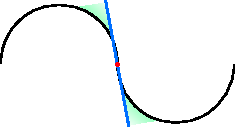
\includegraphics[scale=1.4]{figures/linearizationPoint}
	\caption{Sketch of linearization for the Cubli frame angels.}
	\label{LinearizationSketch}
\end{figure} 
Because we linearize our model there will be an point where the controller no longer will be able to catch the frame, because it cannot predict the forces on the frame anymore. In the sketch of this (see \figref{LinearizationSketch}) the area where the controller will work is indikated by the green area.    %-------- Linearization
\section{Verification of the Model}

To verify the model in simulation \eqref{FrameEq4TaylerApprox} is transformed into the Laplace domain, after which a transfer function of the system is derived. The proceeding equations are valid only around the operating point, and so for better overview, in the following \si{\Delta \theta_F = \theta_F}.
%
\begin{flalign}
	\eq{(J_F+m_w \cdot {l_w}^{2}) \cdot \theta_F \cdot s^2}{-B_F \theta_F\cdot s +  ( m_F \cdot l_F + m_w \cdot l_w ) g \cdot \theta_F - \tau_m + B_w \theta_w\cdot s } \unit{N \cdot m}
\label{LaplaceOfLinearizedModel}
\end{flalign}
%
The angle of the reaction wheel, \si{\theta_w}, still features in \eqref{LaplaceOfLinearizedModel}. It is desireable to have only one input, \si{\tau_m}, and one output, \si{\theta_F}. To achieve this, \eqref{WheelRotEq2} is transformed into the Laplace domain and solved for \si{\theta_w}.
%
\begin{flalign}
	\eq{\theta_w\cdot s^2} {\frac{\tau_m - B_w \theta_w\cdot s}{J_w} - \theta_F\cdot s^2}   &\\
	\eq{\theta_w} {\frac{ -J_w \theta_F \cdot s^2 + \tau_m }{ J_w \cdot s^2 + B_w \cdot s }}&
\label{WheelRotEq2Laplace}
\end{flalign}
%
\Eqref{WheelRotEq2Laplace} is now substituted for \si{\theta_w} in \eqref{LaplaceOfLinearizedModel}, and the transfer function is of the system is derived.
%
\begin{flalign}
	\si{(J_F+m_w \cdot {l_w}^{2}) \cdot \theta_F \cdot s^2} &= \si{-B_F \theta_F\cdot s +  ( m_F \cdot l_F + m_w \cdot l_w ) g \cdot \theta_F - \tau_m} &\nonumber\\
	&\ \ \ \ \si{+ B_w ( \frac{ -J_w \theta_F \cdot s^2 + \tau_m }{ J_w \cdot s^2 + B_w \cdot s } )\cdot s }&
\label{CubliTransferFunction}
\end{flalign}    %-------- Verification

%---------- Chapter 5 ---------------------------------------- Control
%\chapter{System Modelling}
With the given setup being described, it is necessary to study its natural behavior in more details by deriving a model of this system. This chapter shows the process used to put up this model and an analysis of its pertinence. With this model, it shall be possible to determine realistic requirements for the controllers to implement in this project, see \chapref{chap:specifications}.

As a start to this modelling, a mechanical drawing of the Cubli showing angles and coordinate system conventions is seen in \figref{cubliMechanical}. A two-dimensional global coordinate system is chosen with its origin on the pivot point of the frame. Moreover, angles of the total body and the wheel count grow clockwise.

\begin{figure}[H]
 \centering
 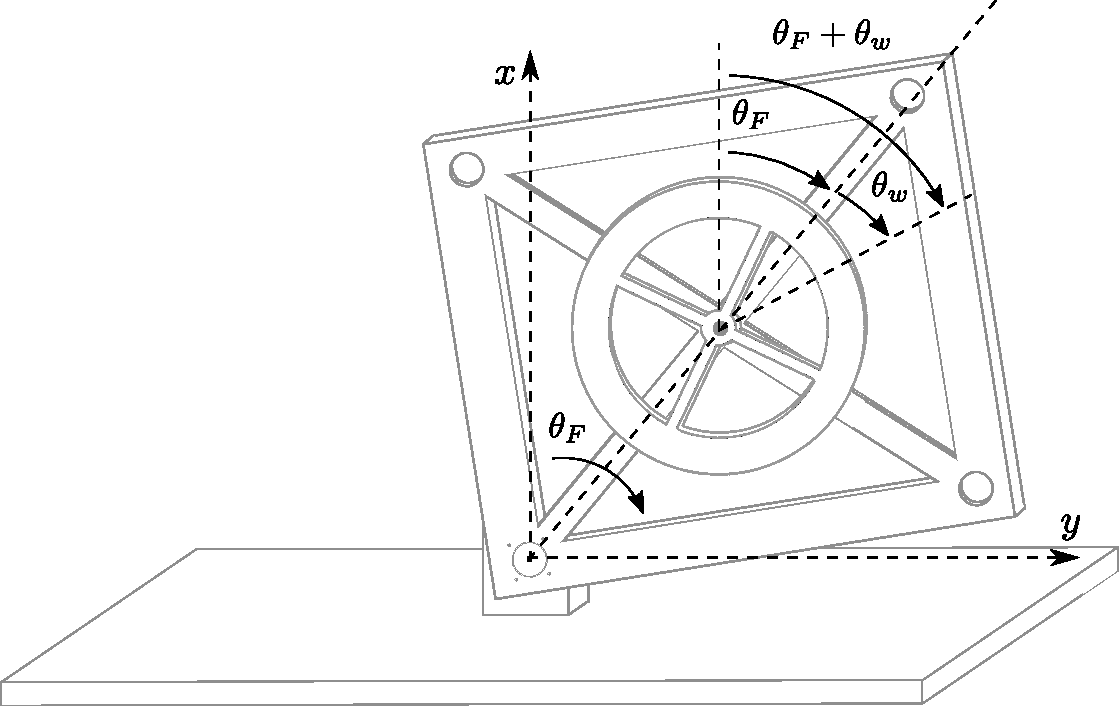
\includegraphics[scale=0.6]{figures/mechanicalSystem}
 \caption{Mechanical drawing of the Cubli, including angle coordinate system conventions}
 \label{cubliMechanical}
\end{figure}

%As shown in \figref{cubliMechanical}, 
In the next section, a complete model of the given setup is derived from Newton's Second Law of motion and rotation.

%%% Part 3 %%%
\part{Test \& Conclusion}
%\chapter{Acceptance Test}
%\chapter{Conclusion}
%\chapter{Discussion}

%%% Setup for Appendix and Bibliography %%%
\bookmarksetup{startatroot}
\addtocontents{toc}{\bigskip}
\newpage
\fancyhead[RO]{\color{aaublue}\small Appendix \nouppercase\rightmark} %even page - chapter title
\fancyhead[LE]{\color{aaublue}\small Appendix \nouppercase\rightmark} %uneven page - section title
\fancyhead[RE,LO]{}
\titleformat{\section}[hang]{\Large\bfseries}{\thesection\hsp\textcolor{aaublue}{|}\hsp}{0pt}{\Large\bfseries}
\renewcommand{\thechapter}{\Alph{chapter}}
\setcounter{chapter}{0}

%%% Appendix %%%
\part*{Appendix}
\addcontentsline{toc}{chapter}{Appendix}

%---------- Appendix A ---------------------------------------- Test Title
\chapter{Verification of the Model}

\textbf{Name: Group 630}\\
\textbf{Date: 07/03 - 2016}

\section*{Purpose}
Compare the response of the real setup with the simulation given by the theoretical model

\section*{Procedure}
\begin{enumerate}
	\item{Turn on the power supply}
	\item{Launch the virtual machine}
	\item{Run Eclipse}
	\item{Set the input current of the motor controller to 0 and change the logfile to store the data}
	\item{Connect the computer to the board through the USB cable}
	\item{Load the changed file in the Beaglebone}
	\item{Keep the Cubli near the vertical position}
	\item{Run the program}
	\item{Let the Cubli fall}
	\item{Stop the program}
	\item{Get the measurements from the file and plot them in Matlab}
	\item{Plot th result of the simulations in the same figure and compare them}
\end{enumerate}

\section*{Results}
\begin{figure}[H] 
	\centering 
	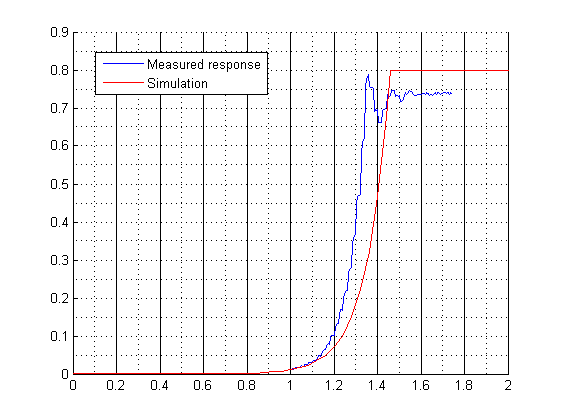
\includegraphics[scale=0.9]{figures/comparisonRealModel}
	\caption{Comparison between the real behavior and the simulation of the linearized model}
	\label{comparisonRealModel}
\end{figure} 

The result of the experiment (\figref{comparisonRealModel}) shows that the response of the real system has several differences with the one from the simulation.

The fist one is the presence of oscillations in the real response curve. This behavior is due to a small bounce that the frame does when it reaches the base.

Another one is the final position of the frame, but it is due to the existence of a piece of foam at this position in the real case (to avoid the Cubli to hit the base).

The other main difference is the shape of the curve, since the simulation is slower than the real case.

\section*{Conclusions}



%---------- Appendix B ---------------------------------------- Test Title
%\chapter{Impulse Response}\label{impulseTestAppendix} 
\textbf{Name: Group 630}\\
\textbf{Date: 11/03 - 2016}

\subsubsection{Purpose}
To observe the impulse response of the Cubli hanging upside down.

Data is used to compare the response of measured response and the simulation given by the theoretical nonlinear model.

\subsubsection{Setup}
The Cubli is put upside down under a table with 2 clamps placed at each side of the bottom plate of the Cubli setup.
The wheel is being held in a fixed position with a strip tied to it and the frame. The probe chosen is a 1:1 and is connected to the potentiometer with probe to yellow cable and ground clamp to brown cable. The power supply has to be connected, and turned on, to the Cubli in order to get readouts from the potentiometer.
\begin{figure}[H] 
	\centering 
	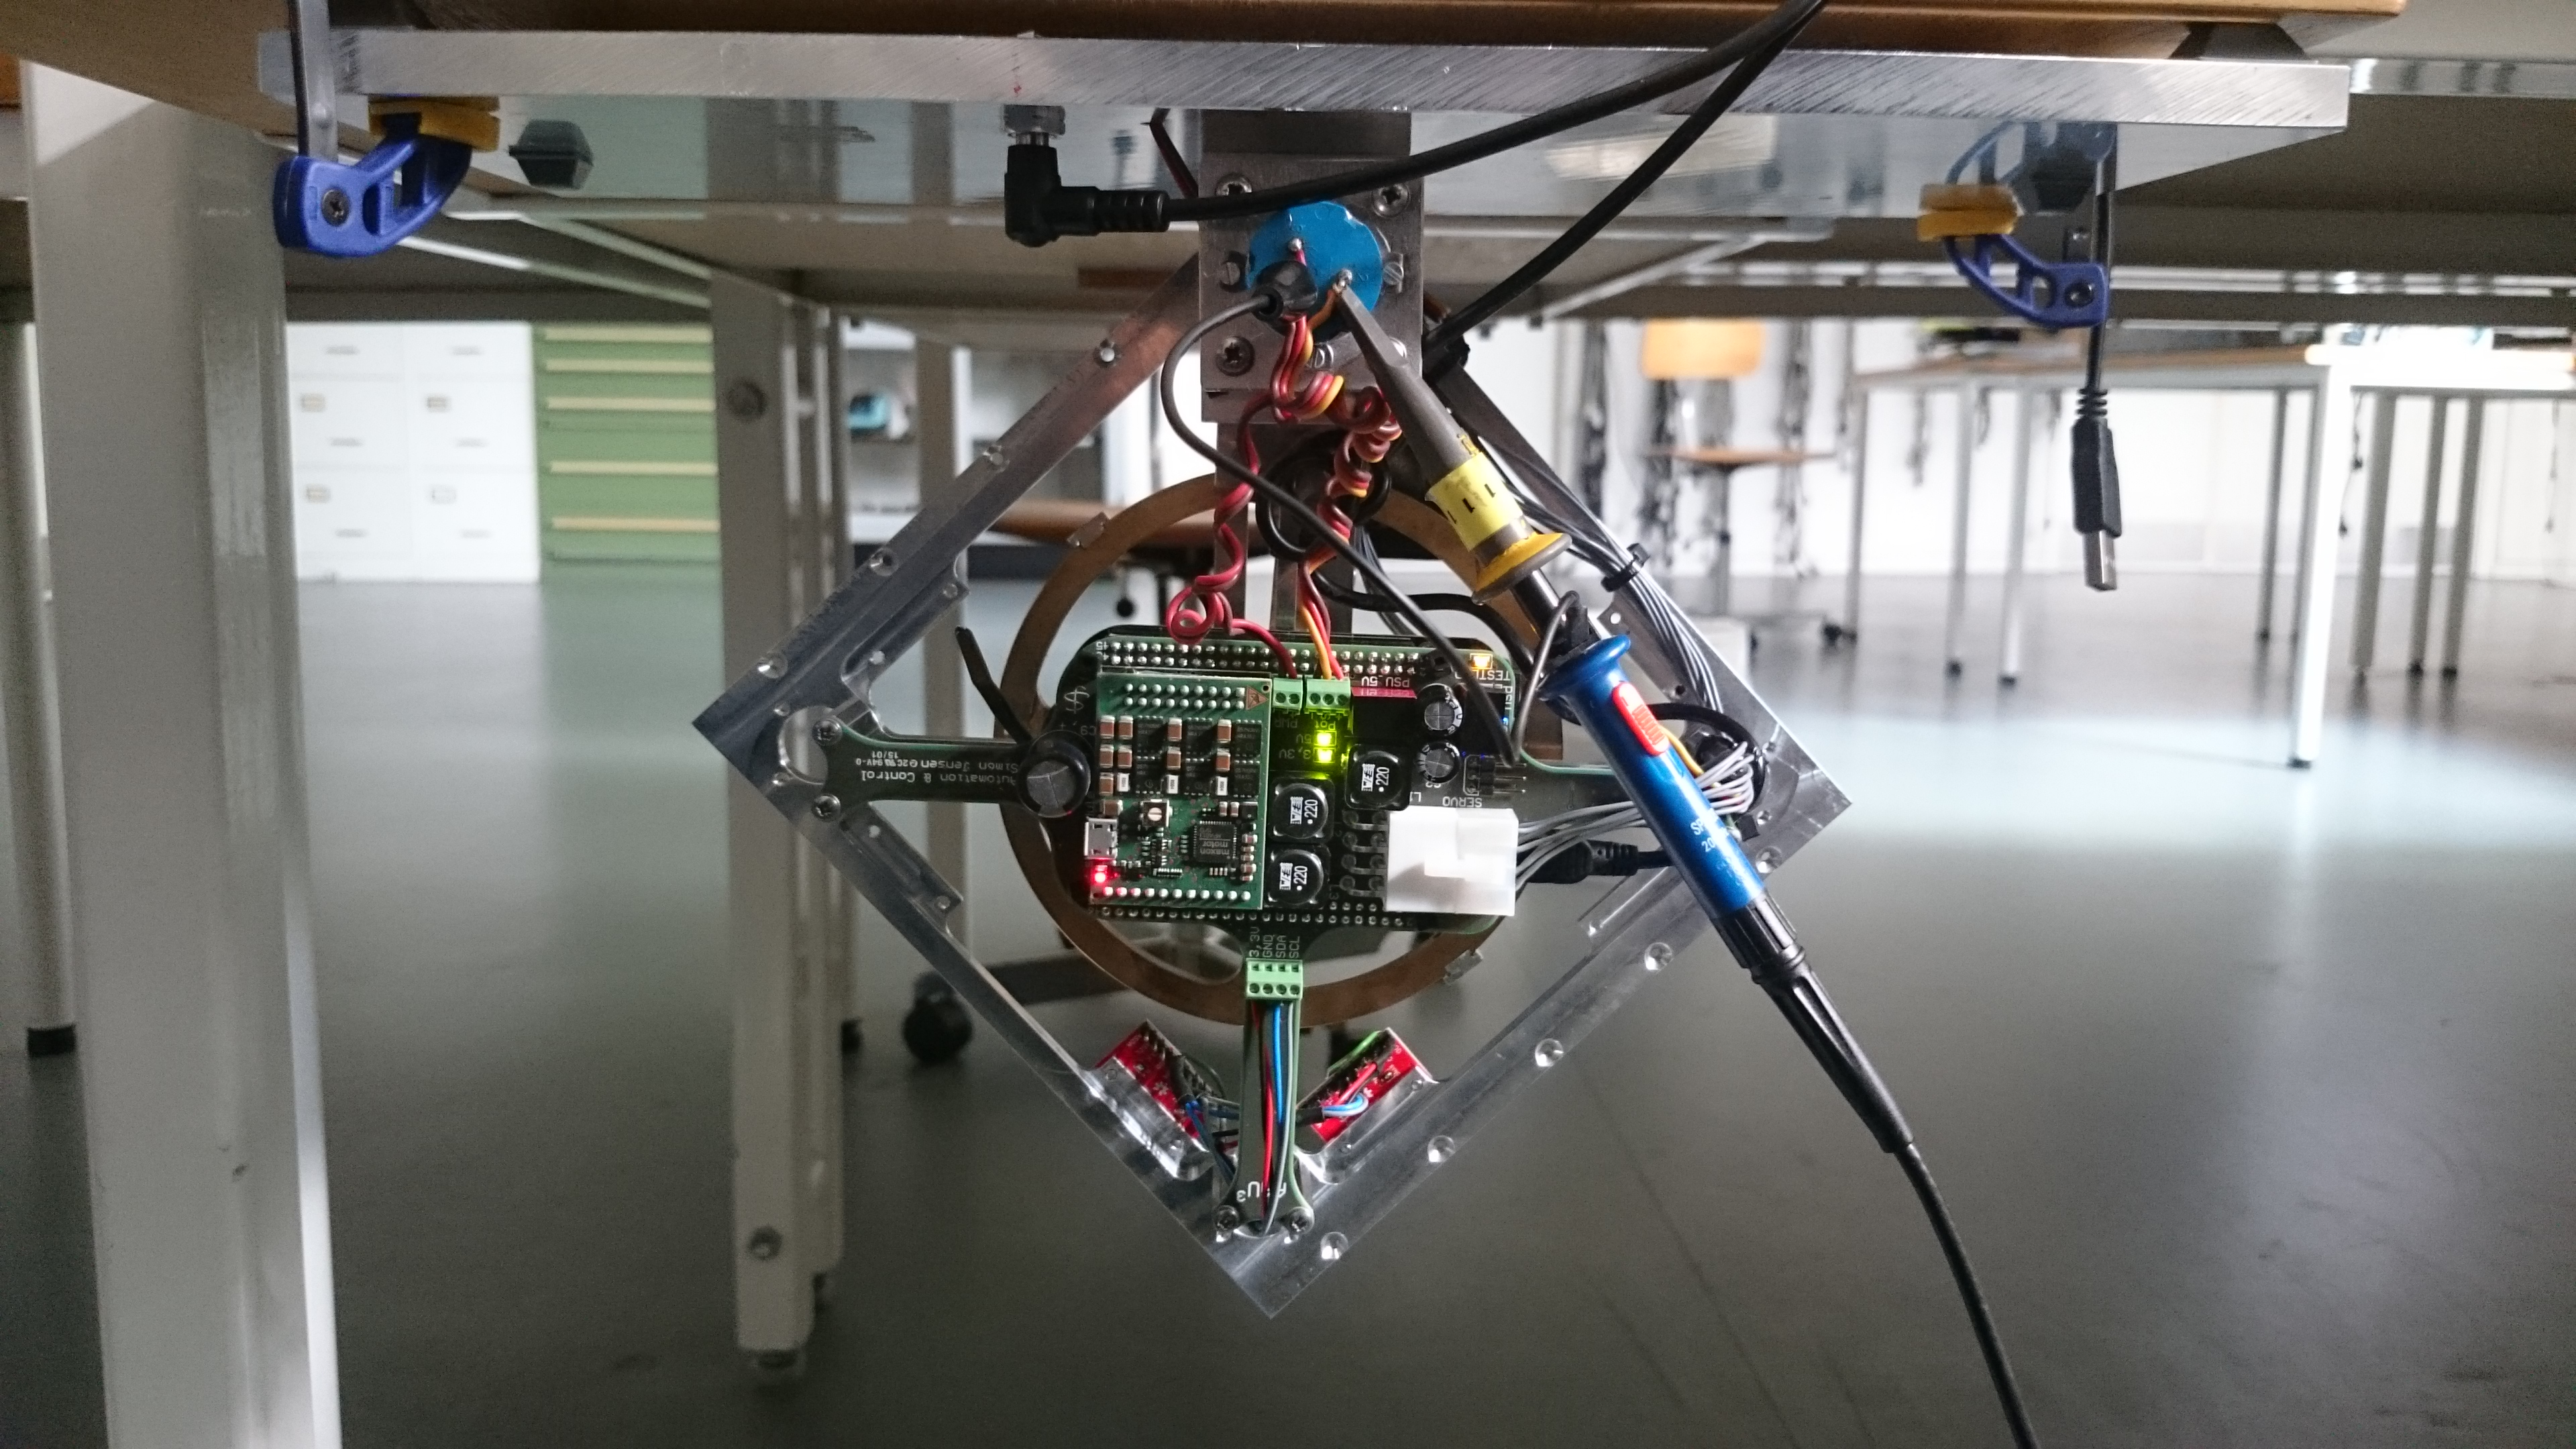
\includegraphics[scale=0.08]{figures/impulseResponseSetup}
	\caption{The Cubli setup hanging upside down beneath a table during the impulse response test}
	\label{impulseResponseTestPicture}
\end{figure} 

\subsubsection{List of Equipment}
\begin{table}[H]
	\begin{tabular}{|l|l|p{4cm}|}
		\hline%------------------------------------------------------------------------------------
		\textbf{Instrument}                        &  \textbf{AAU-no.}  &  \textbf{Type}       \\
		\hline%------------------------------------------------------------------------------------
		Cubli setup                              &               &  		  					\\
		\hline%------------------------------------------------------------------------------------
		Oscilloscope                              &  61604             &  Agilent 54621A		  \\
		\hline%------------------------------------------------------------------------------------
		Dedicated Power Supply of Cubli \small{(24 V - 3 A)} &               &  XP Power, AEB70US24 \\
		\hline%------------------------------------------------------------------------------------
		Probe 1:1                &  TBD            		&          TBD\fxnote{find the probe used}  \\
		\hline%------------------------------------------------------------------------------------
		2x Clamp                &  			            &          							   \\
		\hline%------------------------------------------------------------------------------------
	\end{tabular}
\end{table}

\subsubsection{Procedure}
\begin{enumerate}
	%\item Turn on the power supply
	\item Place the setup upside-down and place the frame touching the base %, \si{135^0} with respect to the vertical position
	\item Let the Cubli fall and swing until it has come to rest
	\item Use the oscilloscope to measure the changes in the potentiometer
	\item Collect all the data and plot it in Matlab
%	\item Compare with the simulation 
	
\end{enumerate}

\subsubsection{Results}
\begin{figure}[H] 
	\centering 
	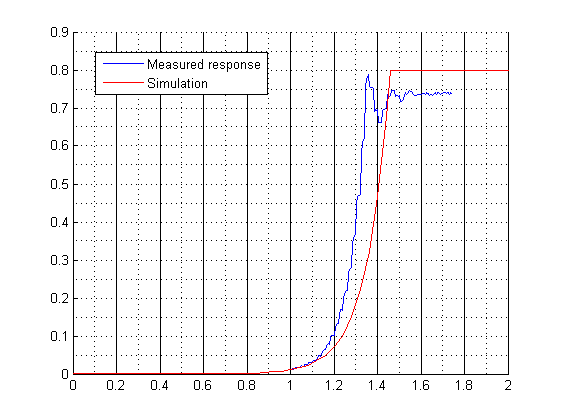
\includegraphics[scale=0.9]{figures/comparisonRealModel}
	\caption{Comparison between the real behavior and the simulation of the linearized model}
	\label{comparisonRealModel}
\end{figure} 

\subsubsection{Note}
During this experiment it was observed that if the frame was released from the left position (The right upper side on \figref{impulseResponseTestPicture} since the Cubli is upside down) that the frame would hit the rubber pad on the other side. This behavior was not observed when releasing the Cubli from the right position (left upper corner).

\subsubsection{Conclusions}

%----------Appendix C ---------------------------------------- Test Title
%\chapter{Test}

%---------- Appendix D ---------------------------------------- Test Title
%\chapter{Test}

%%% Bibliography %%%
\printbibliography

%%% To Do List %%%

\end{document}
